\chapter{Implementation and hosting}
\lhead{\textit{Chapter \thechapter}}
\rhead{\textit{Implementation and hosting  }}

\section{Introduction}
After completing the application design arrange, in this chapter we'll begin the implementation and assessment arrange by displaying the work environments and innovation utilized in creating the application, which made it conceivable to reach the ultimate result, and we'll also display the interfacing whereas actualizing the application capacities, and at the conclusion we provide an clarification of the foremost critical highlights of the application. \\


\section{Work environement}
This project was built up on distinctive work environement, agreeing to the available capabilities in arrange to reach the most excellent conceivable result. These environments are:\\

\subsection{Hardware}
For programming we used a laptop, as for testing we used mobile phones, laptops, tabeltes and even a smart tv to monitor the performance of the website on them. The characteristics of
these devices are:
\begin{itemize}
	\item LENOVO ThinkPad T470s laptop(for programming):
	\begin{itemize}
		\item Processor : Intel (R) Core (TM) i7-7600U CPU @ 2.80 GHz(4 CPUs), ~2.90 GHz.
		\item RAM : 16 GB.
		\item System : Windows 10 Pro - 64 Bit.
	\end{itemize}
\end{itemize}

\begin{itemize}
	\item HP ProBook 640 G1 laptop(for testing):
	\begin{itemize}
		\item Processor : Intel (R) Core (TM) i7-4600M CPU @ 2.90 GHz(4 CPUs), ~2.90 GHz.
		\item RAM : 8 GB.
		\item System : Windows 10 Pro - 64 Bit.
	\end{itemize}
\end{itemize}

\begin{itemize}
	\item LATITUDE 3330 laptop(for testing):
	\begin{itemize}
		\item Processor : Intel (R) Core (TM) i5-3337U CPU @ 1.80 GHz, 1.80 GHz.
		\item RAM : 12.0 GB.
		\item System : Windows 10 Pro - 64 Bit.
	\end{itemize}
\end{itemize}

\begin{itemize}
	\item SamSung Galaxy J2 phone(for testing):
	\begin{itemize}
		\item RAM : 1 GB.
		\item System : Android 5.1.1.
	\end{itemize}
\end{itemize}

\begin{itemize}
	\item SamSung Galaxy M20 phone(for testing):
	\begin{itemize}
		\item RAM : 3 GB.
		\item System : Android 10.
	\end{itemize}
\end{itemize}



\subsection{Software}

\textbf{\noindent	Visual Studio Code:\\}
\indent Visual Studio Code is not just another evolved Notepad with syntax colorization and automatic indentation. Instead, it is a very powerful code-focused development
 environment expressly designed to make it easier to write web, mobile, and cloud applications using languages that are available to different development platforms and
  to support the application development life cycle with a built-in debugger and integrated support for the popular Git version control engine.\cite{Del_Sole2021-cv}\\

\textbf{\noindent Sublime Text:\\}
\indent Sublime Text is a proprietary, cross-platform text editor designed for people who spend huge amounts of time shuffling code around. A programmer's editor,
 Sublime Text is a third option to the long-standing “Vi or Emacs” conundrum. Going beyond the basics of syntax highlighting and code folding, Sublime offers a 
 litany of innovative and unique features. With version 3.0 just around the corner, I'm taking you on a tour of Sublime's most compelling features and add-on packages.\cite{kinder2013sublime}\\


 \textbf{\noindent XAMPP:\\}
 \indent XAMPP is a small and light Apache distribution containing the most common web development
 technologies in a single package. Its contents, small size, and portability make it the ideal tool for
 students developing and testing applications in PHP and MySQL. XAMPP is available as a free
 download in two specific packages: full and lite. While the full package download provides a wide
 array of development tools, this article will focus on using XAMPP Lite which contains the necessary
 technologies that meet the Ontario Skills Competition standards. As the name implies, the light version
 is a small package containing Apache HTTP Server, PHP, MySQL, phpMyAdmin, Openssl, and
 SQLite.\cite{dvorski2007installing}\\



\newpage


\section{Used programming languages}


\subsection{HTML: HyperText Markup Language}
HTML (HyperText Markup Language) is the most basic building block of the Web. It defines the meaning and structure of web content. Other technologies besides HTML are generally used to describe a web page's appearance/presentation (CSS) or functionality/behavior (JavaScript).\cite{MDN-HTML}\\

\subsection{CSS: Cascading Style Sheets}
Cascading Style Sheets (CSS) is a stylesheet language used to describe the presentation of a document written in HTML or XML (including XML dialects such as SVG, MathML or XHTML). CSS describes how elements should be rendered on screen, on paper, in speech, or on other media.\cite{MDN-CSS}\\

\subsection{JavaScript — Dynamic client-side scripting}
JavaScript is a programming language that allows you to implement complex things on web pages. Every time a web page does more than just sit there and display static information for you to look at—displaying timely content updates, interactive maps, animated 2D/3D graphics, scrolling video jukeboxes, or more—you can bet that JavaScript is probably involved.\cite{MDN-JS}\\

\subsection{MySQL — Structured Query Language}
MySQL is a very fast, robust, relational database management system. A database enables you to efficiently store, search, sort, and retrieve data. The MySQL server controls access to your data to ensure that only authorized users can obtain access. Hence, MySQL is a multi-user, multi-threaded server. It uses SQL the standard database query language worldwide.\cite{welling2003php}




\section{Presentation of graphical interfaces}


\subsection{Home page interface}
When the client visit the website, the first thing he sees is the home page. fig \ref{fig:Homepage1}\\
\footnote[2]{The website is responsive so will show it in desktop and mobile\cite{noauthor_undated-an}}

\textbf{On Desktop:}
%***************************************************
\begin{figure*}[ht]
	\centering
	\label{}
\includegraphics[scale=0.5]{img/0.jpg}                
	\caption{Home page} 
	\label{fig:Homepage1}
\end{figure*} 
%===================================================================


%***************************************************
\begin{figure*}[ht]
	\centering
	\label{}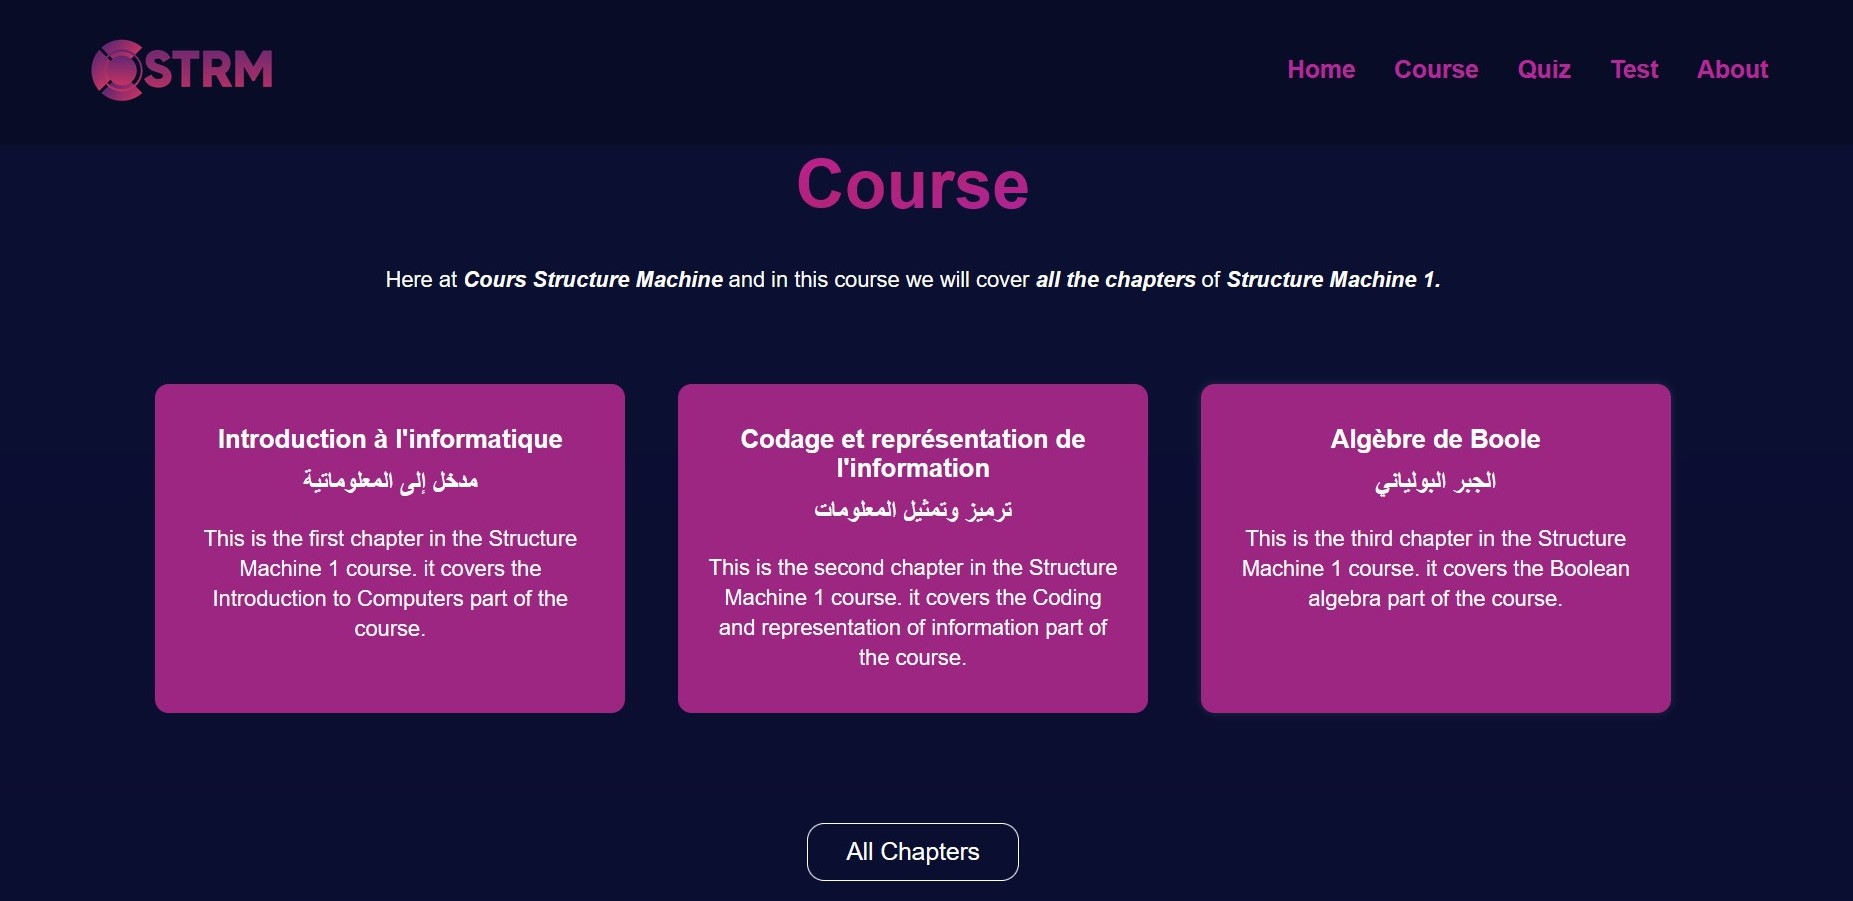
\includegraphics[scale=0.5]{img/1.jpg}                
	\caption{Home page} 
	\label{fig:Homepage2}
\end{figure*} 
%===================================================================
%***************************************************
\begin{figure*}[ht]
	\centering
	\label{}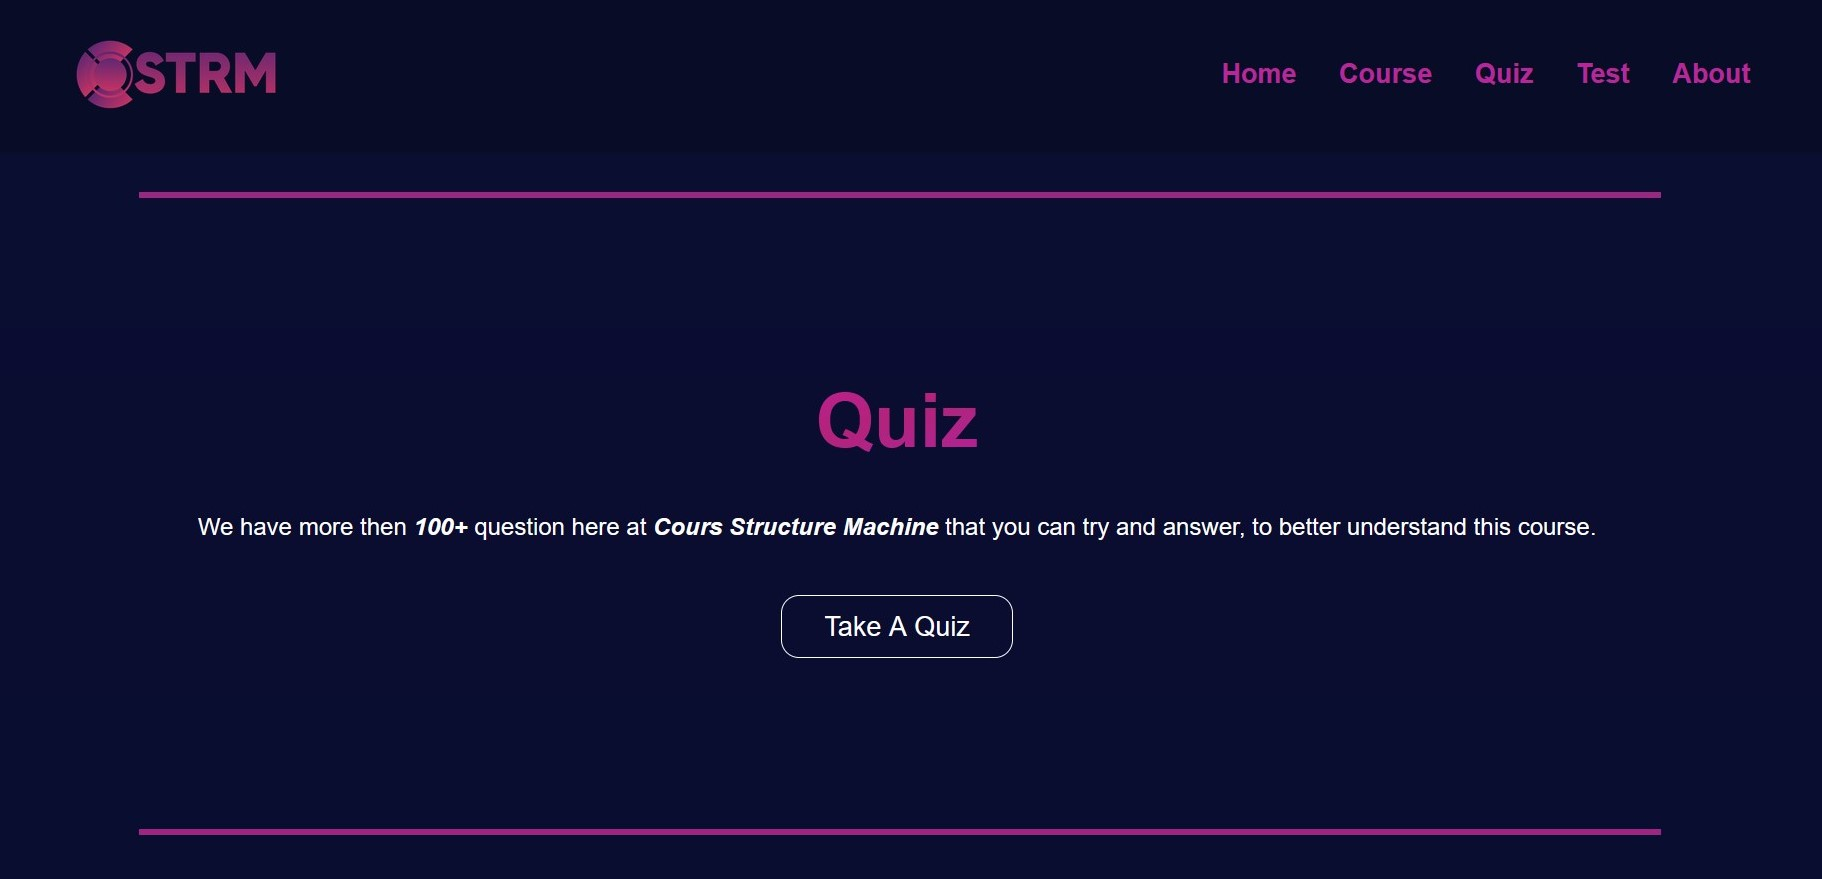
\includegraphics[scale=0.5]{img/2.jpg}                
	\caption{Home page} 
	\label{fig:Homepage3}
\end{figure*} 
%===================================================================
\textbf{On Mobile:}
\begin{figure*}[ht]
	\centering
	\label{}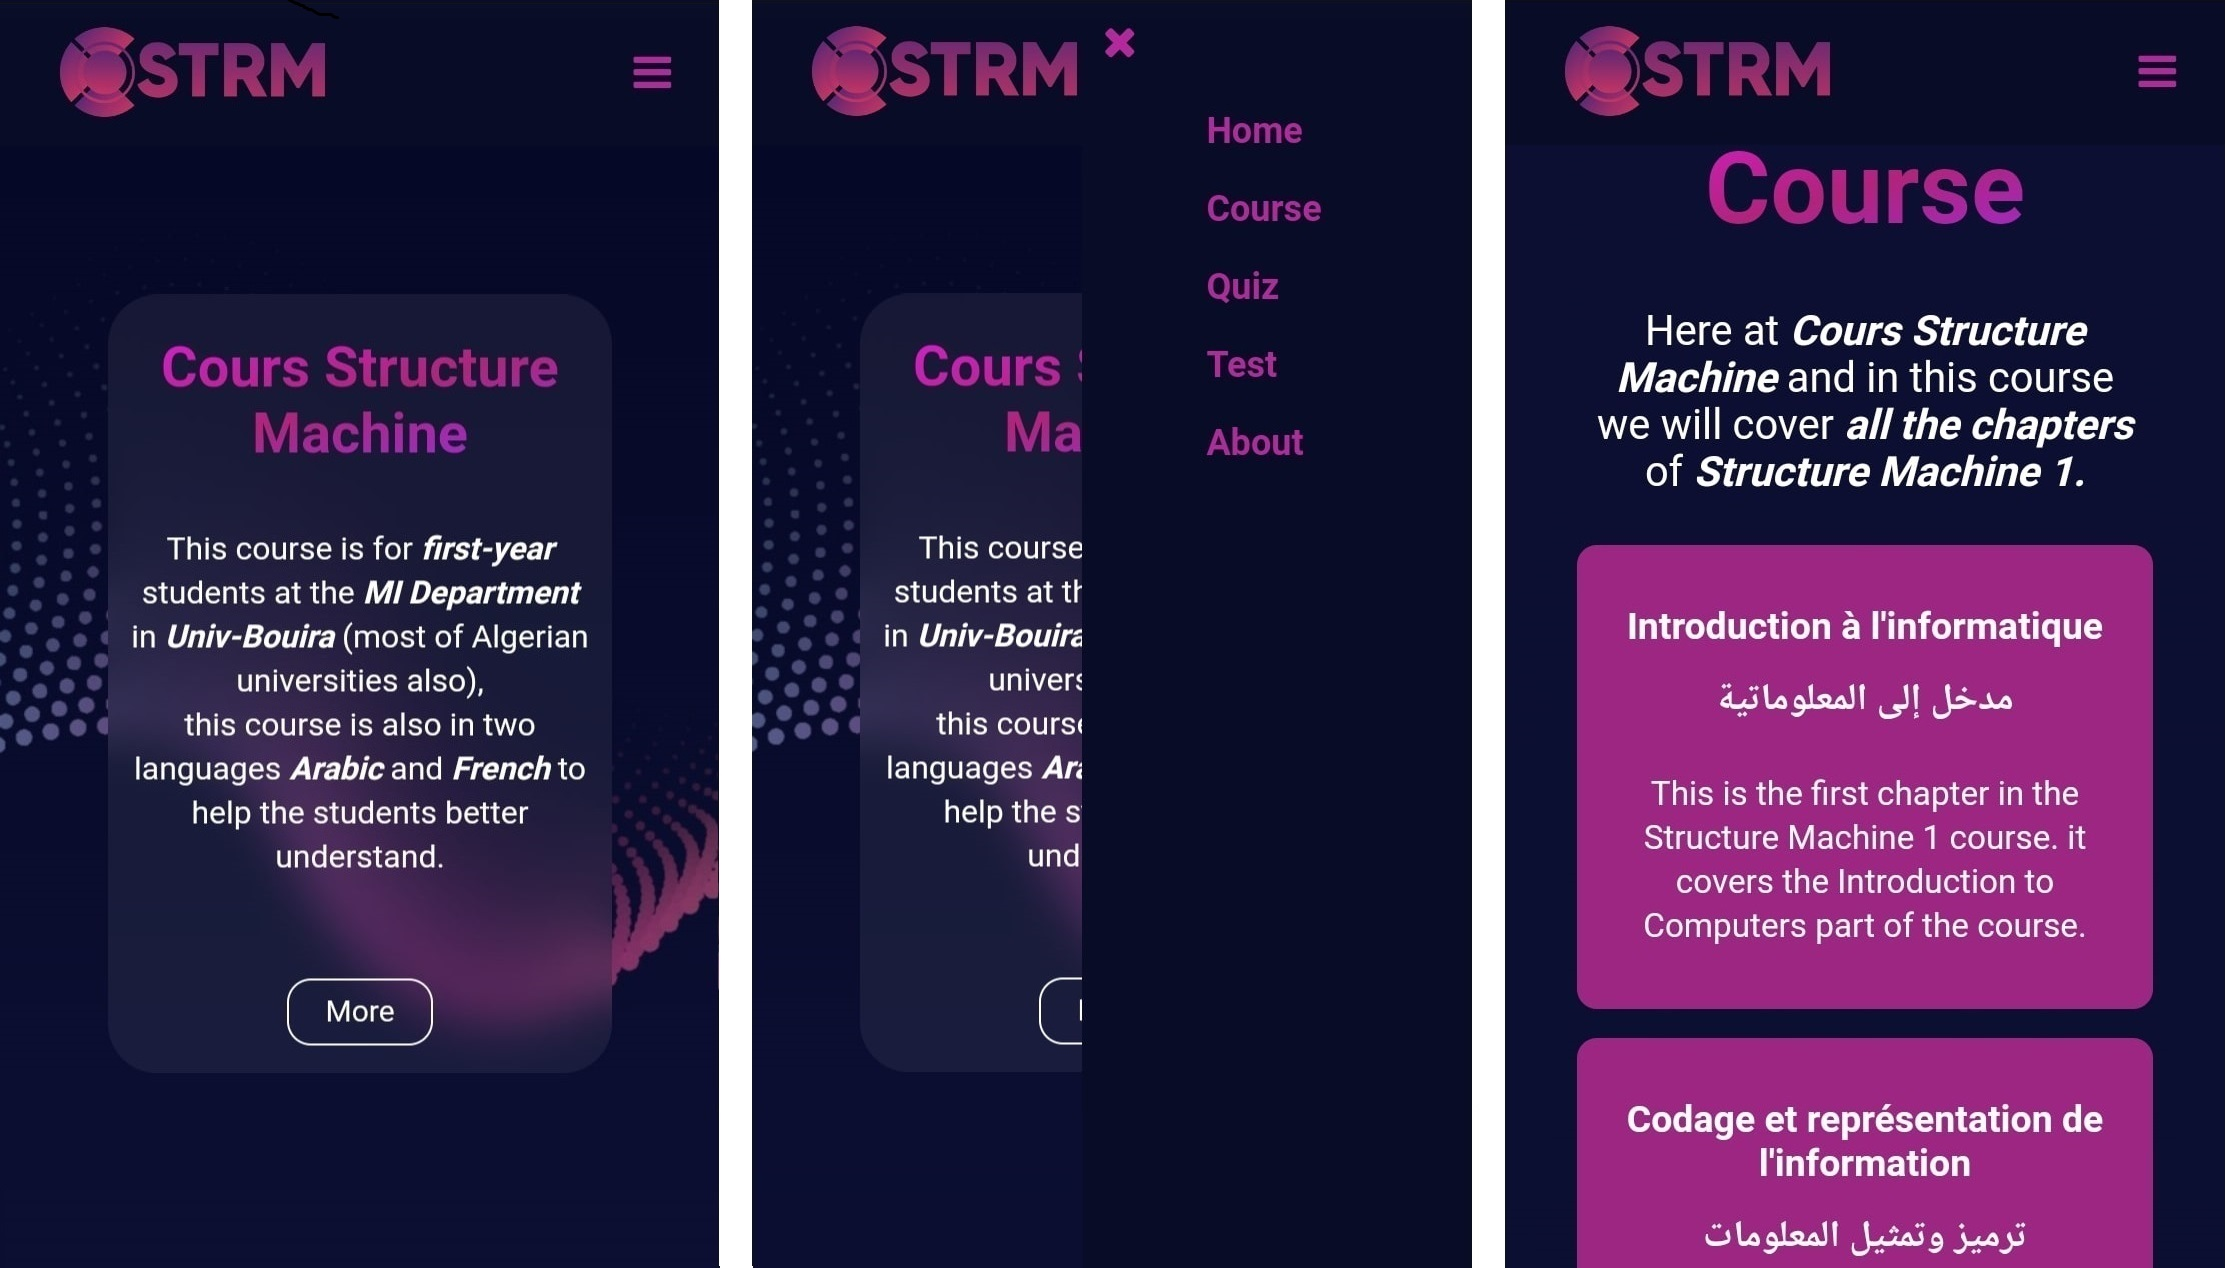
\includegraphics[scale=0.249]{img/00000.jpg}                
	\caption{Home page} 
	\label{fig:Homepage4}
\end{figure*}

\newpage

\subsection{Course page interface}
The user(client) will find the course in the course page, the course page have a local navigation (see figure \ref{fig:coursepage1}), it is also in two languages (see figure \ref{fig:coursepage3})\\
\textbf{On Desktop:}
%***************************************************
\begin{figure*}[ht]
	\centering
	\label{}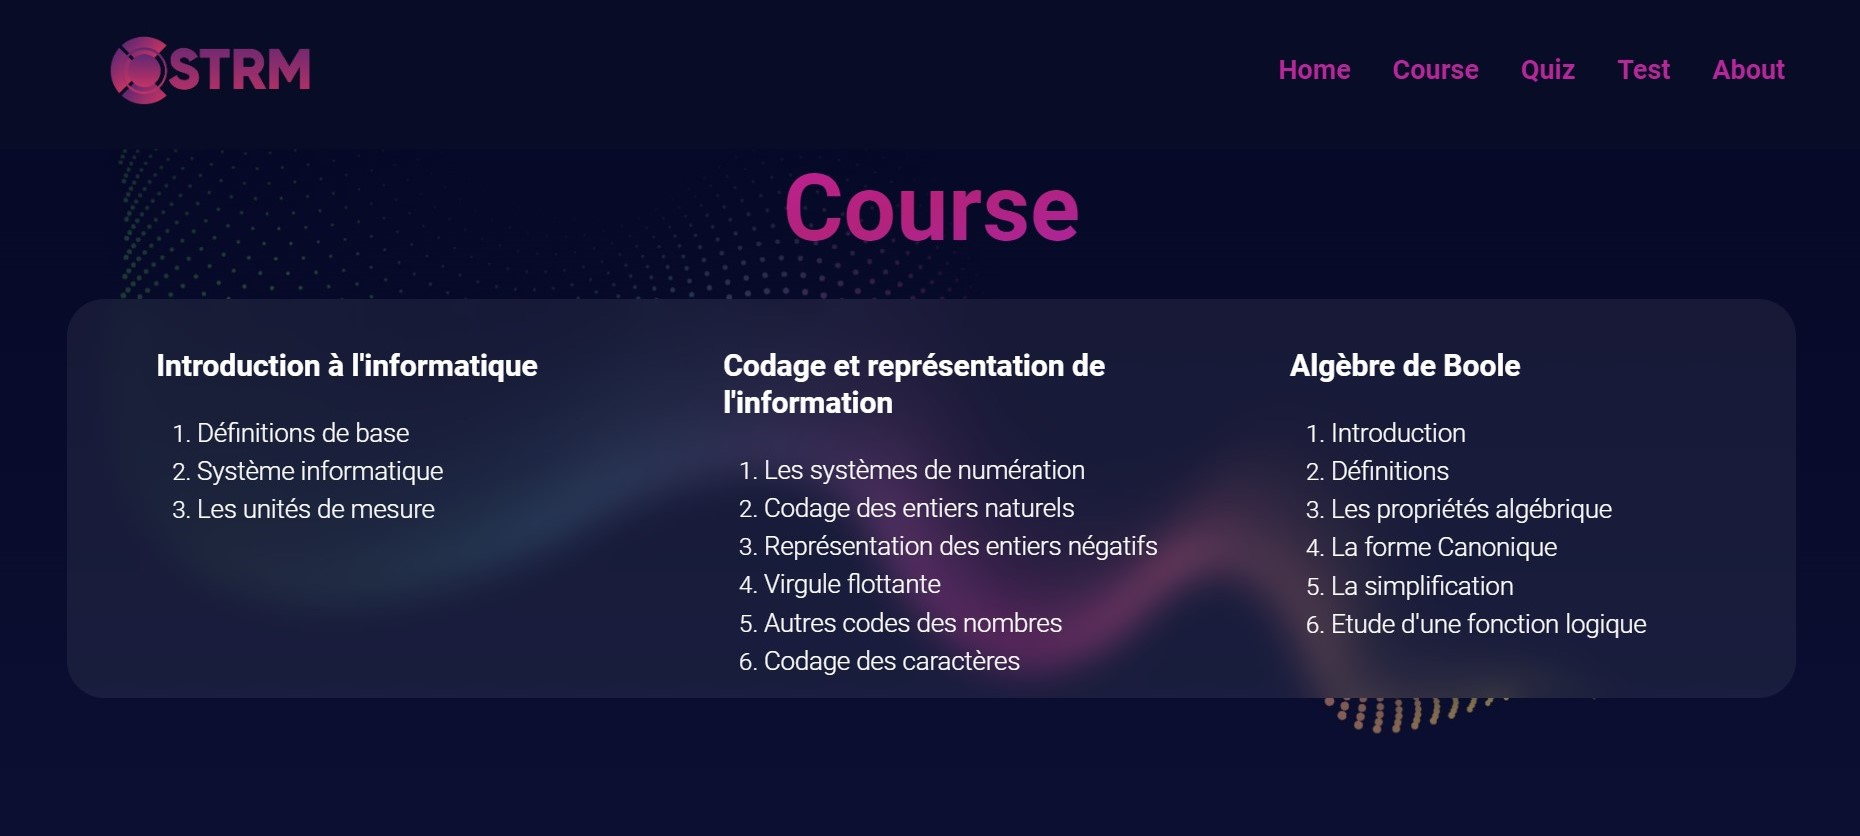
\includegraphics[scale=0.5]{img/3.jpg}                
	\caption{Course page} 
	\label{fig:coursepage1}
\end{figure*} 
%===================================================================


%***************************************************
\begin{figure*}[ht]
	\centering
	\label{}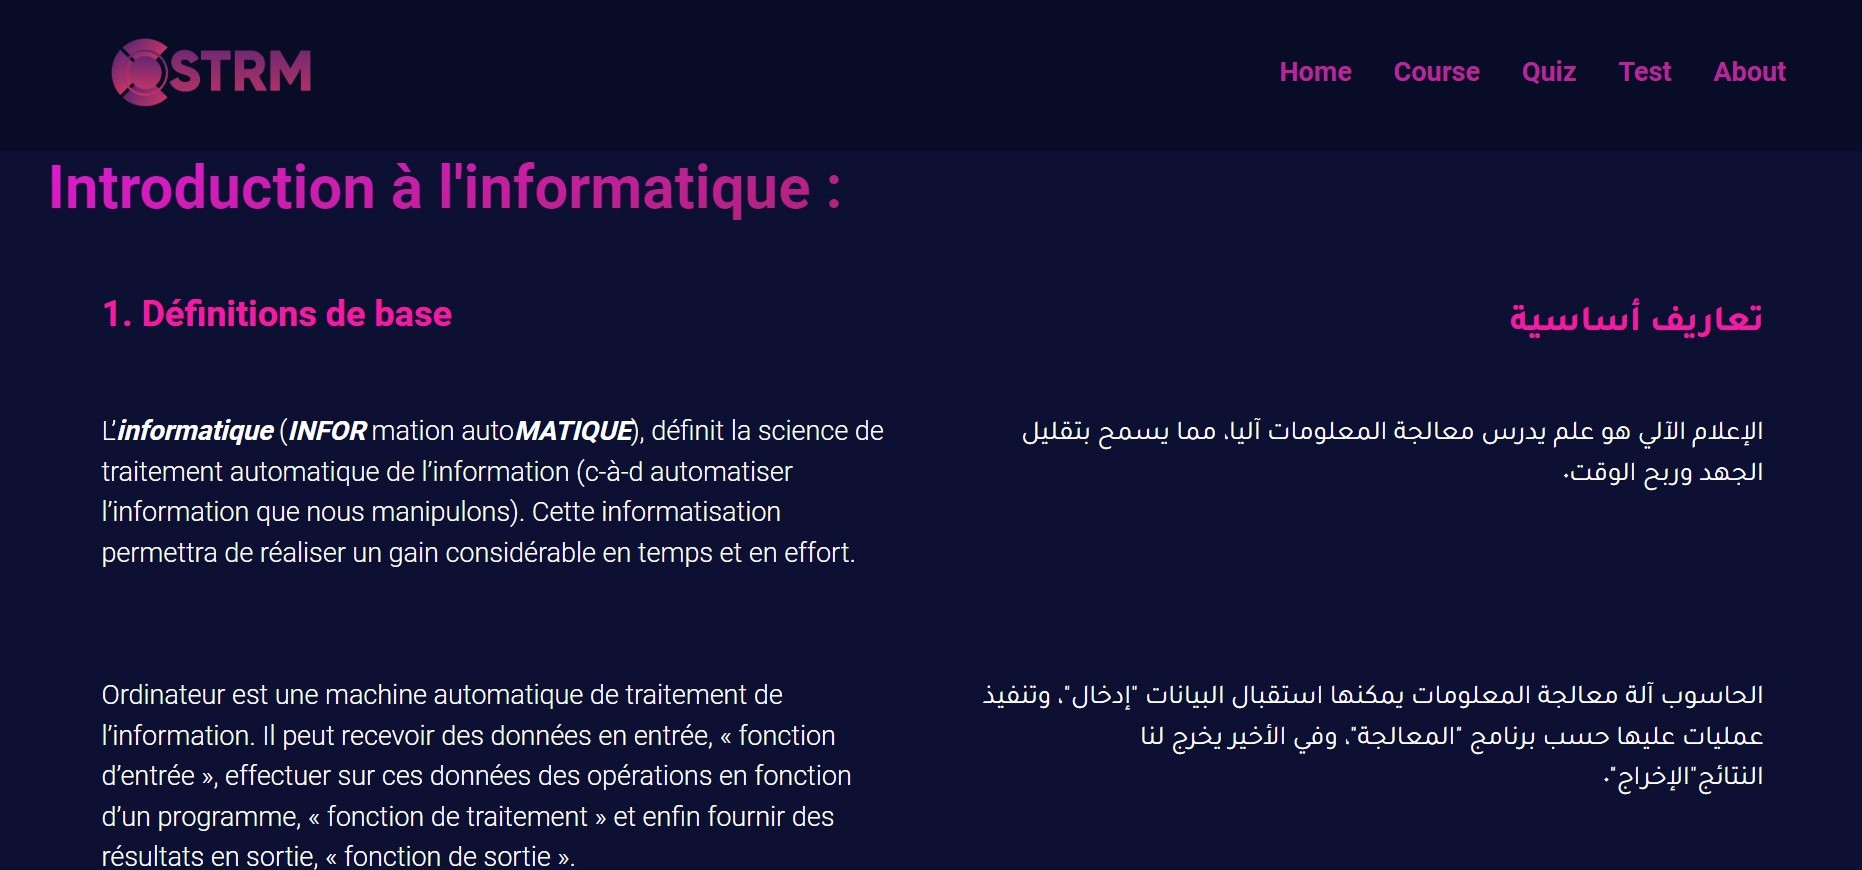
\includegraphics[scale=0.5]{img/4.jpg}                
	\caption{Course page} 
	\label{fig:coursepage2}
\end{figure*} 
%===================================================================

\newpage

%***************************************************
\begin{figure*}[ht]
	\centering
	\label{}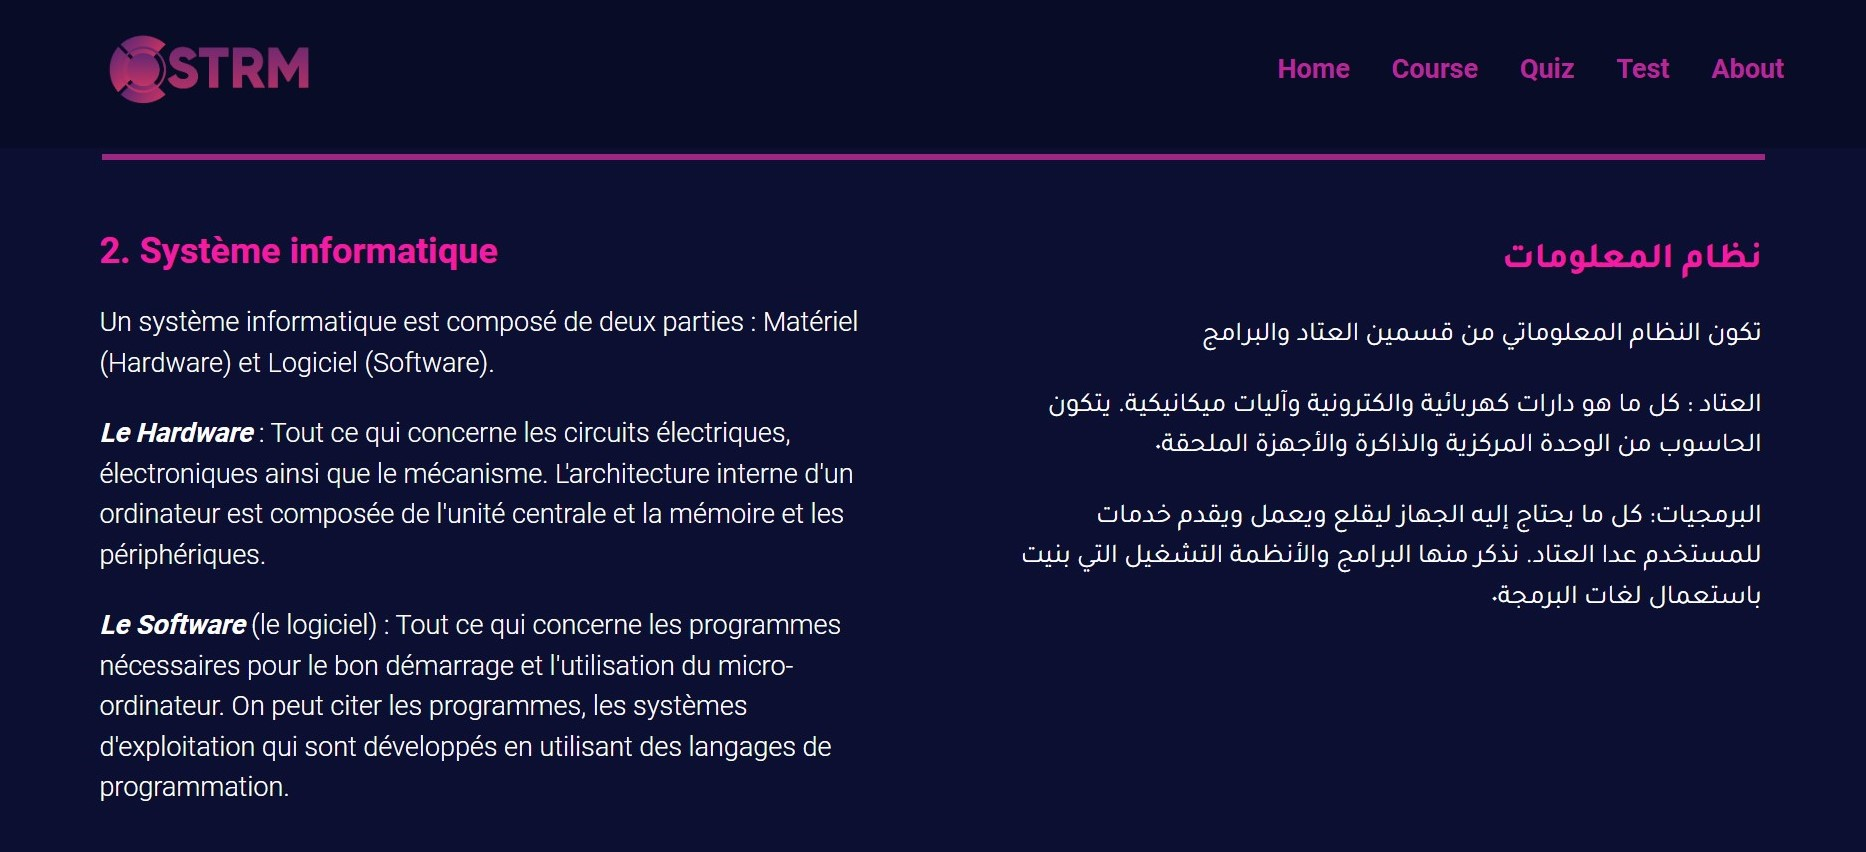
\includegraphics[scale=0.5]{img/5.jpg}                
	\caption{Course page} 
	\label{fig:coursepage3}
\end{figure*}  
%===================================================================

%***************************************************
\begin{figure*}[ht]
	\centering
	\label{}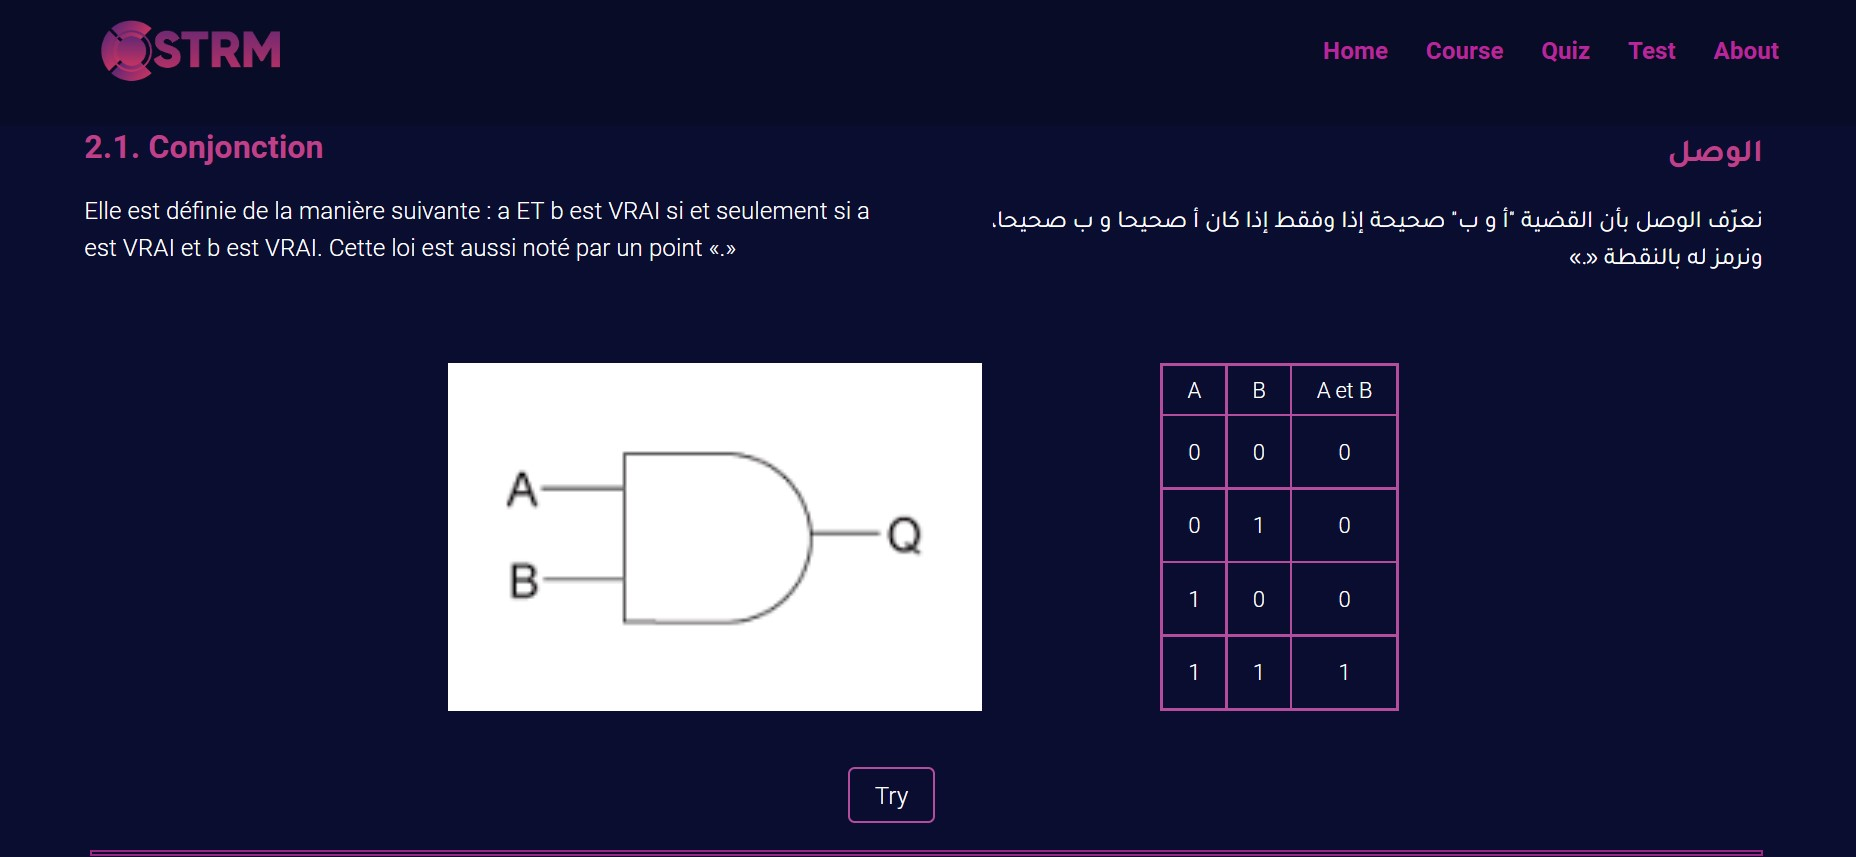
\includegraphics[scale=0.5]{img/14.jpg}                
	\caption{Course page} 
	\label{fig:coursepage4}
\end{figure*} 
\newpage
%===================================================================
\textbf{On Mobile:}
\begin{figure*}[ht]
	\centering
	\label{}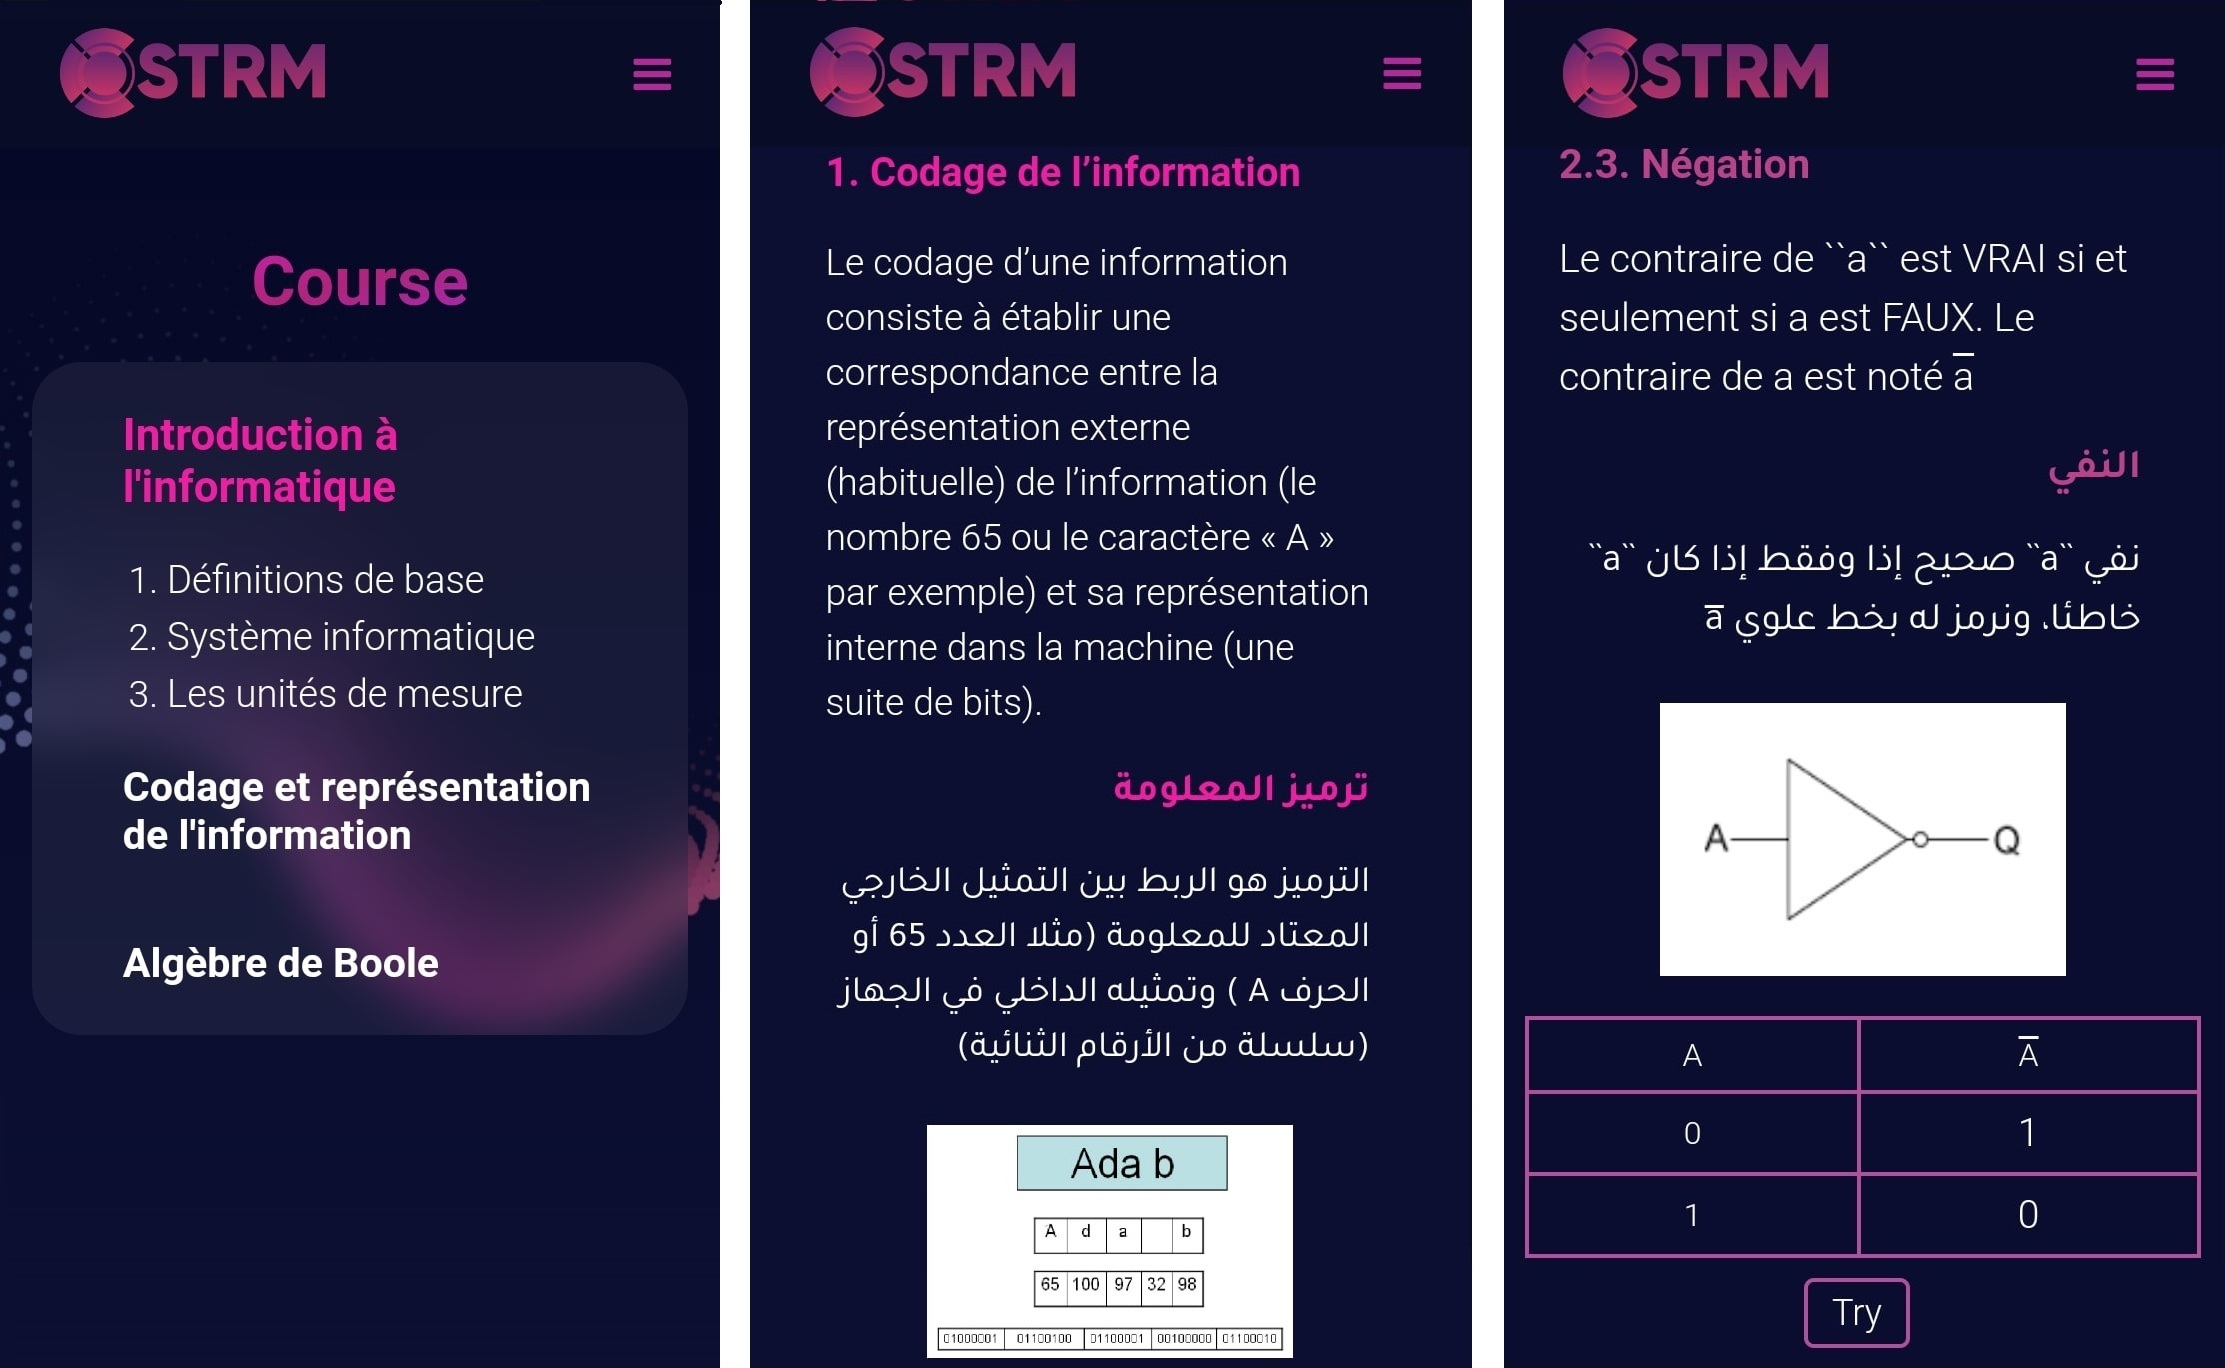
\includegraphics[scale=0.3]{img/22222.jpg}                
	\caption{Home page} 
	\label{fig:Homepage5}
\end{figure*}


\subsection{Try interface}
The objective of this project is to make an interactive couse, so we gave the user the option to try and test his knowledge(see figure \ref{fig:try1}, \ref{fig:try2}, \ref{fig:try3})\\\\
\textbf{On Desktop:}
%***************************************************
\begin{figure*}[ht]
	\centering
	\label{}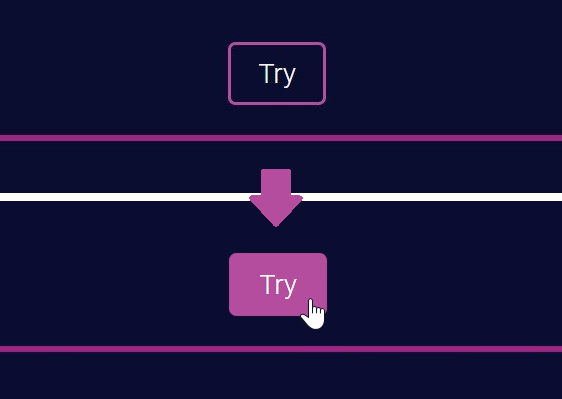
\includegraphics[scale=0.6]{img/13.png}                
	\caption{Try option} 
	\label{fig:try1}
\end{figure*} 
%===================================================================


%*************************************************
%===================================================================

\newpage

%***************************************************
\begin{figure*}[ht]
	\centering
	\label{}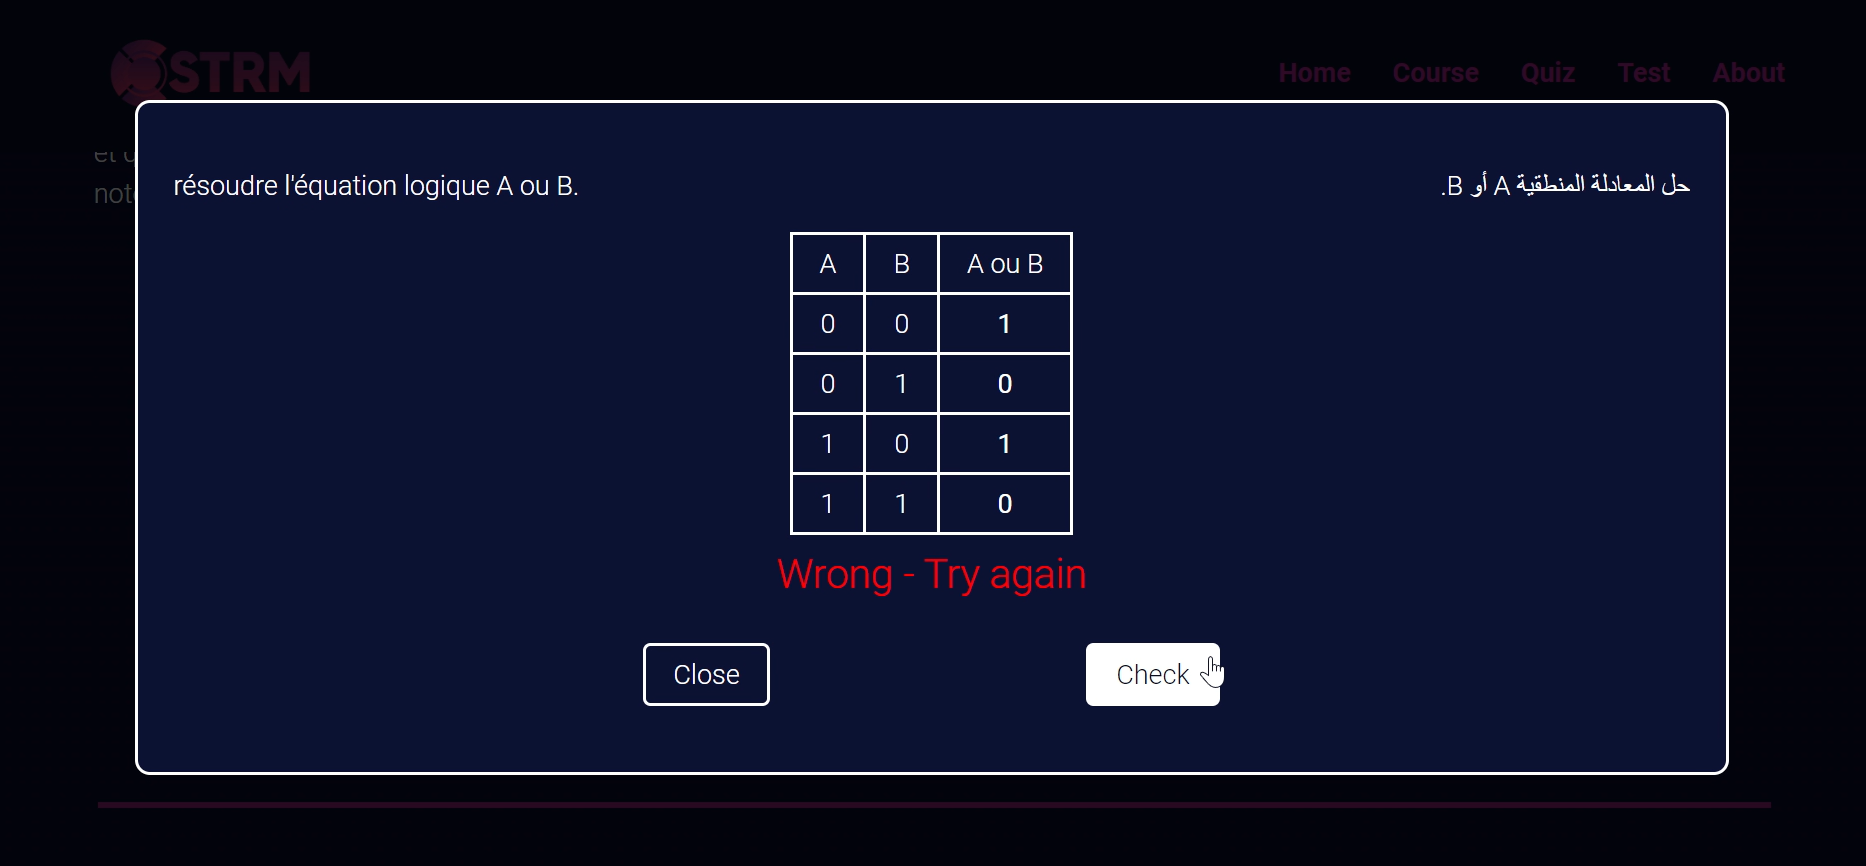
\includegraphics[scale=0.5]{img/11.png}                
	\caption{Try option} 
	\label{fig:try2}
\end{figure*} 
%===================================================================


%***************************************************
\begin{figure*}[ht]
	\centering
	\label{}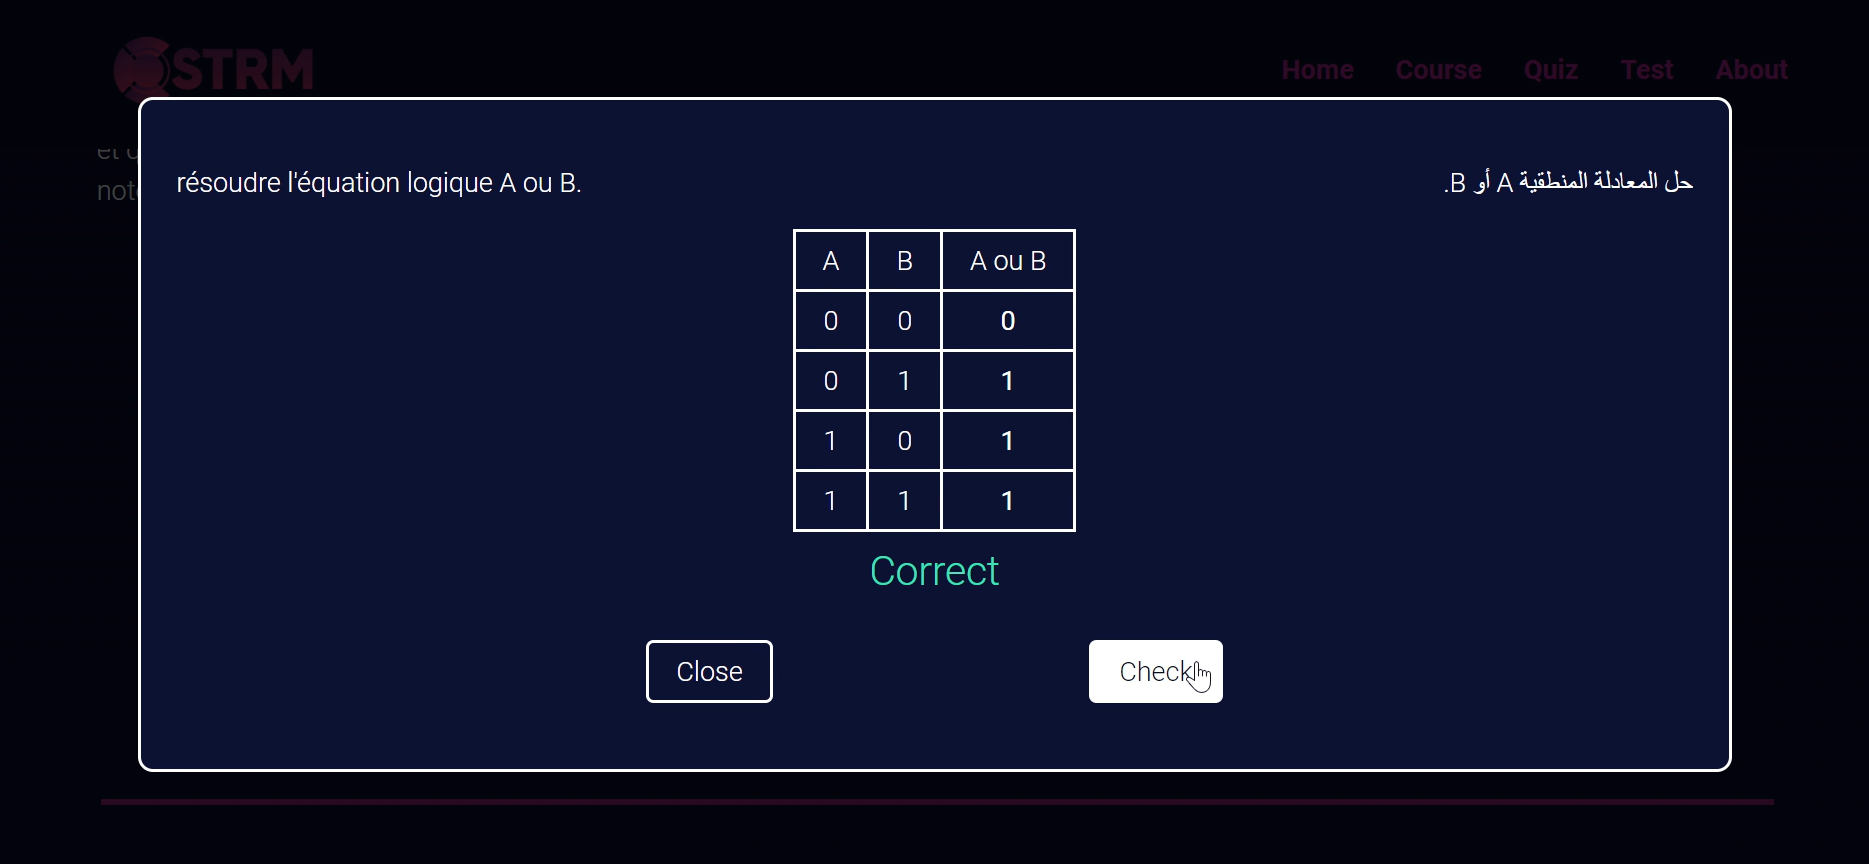
\includegraphics[scale=0.5]{img/12.png}                
	\caption{Try option} 
	\label{fig:try3}
\end{figure*} 
%===================================================================
\newpage

\textbf{On Mobile:}
\begin{figure*}[ht]
	\centering
	\label{}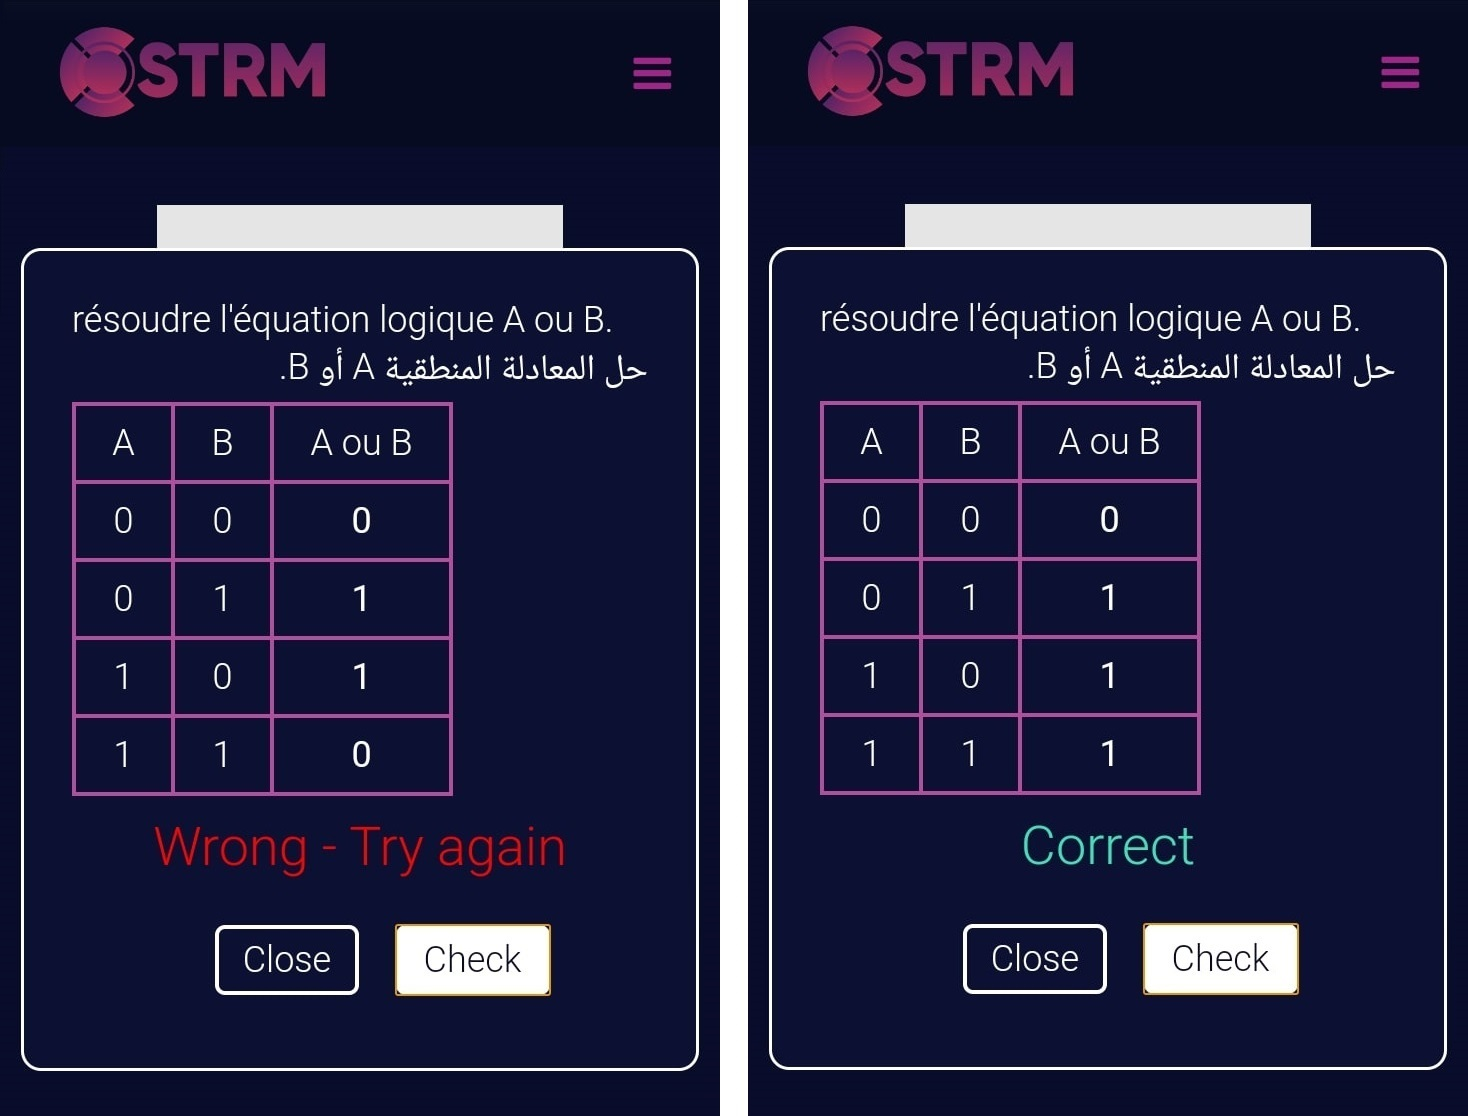
\includegraphics[scale=0.45]{img/333.jpg}                
	\caption{Try option} 
	\label{fig:try4}
\end{figure*}
\newpage
\subsection{Quiz interface}
The quiz is where the user can test his knowledge with random questions(see figure \ref{fig:quiz})
\begin{figure*}[ht]
	\centering
	\label{}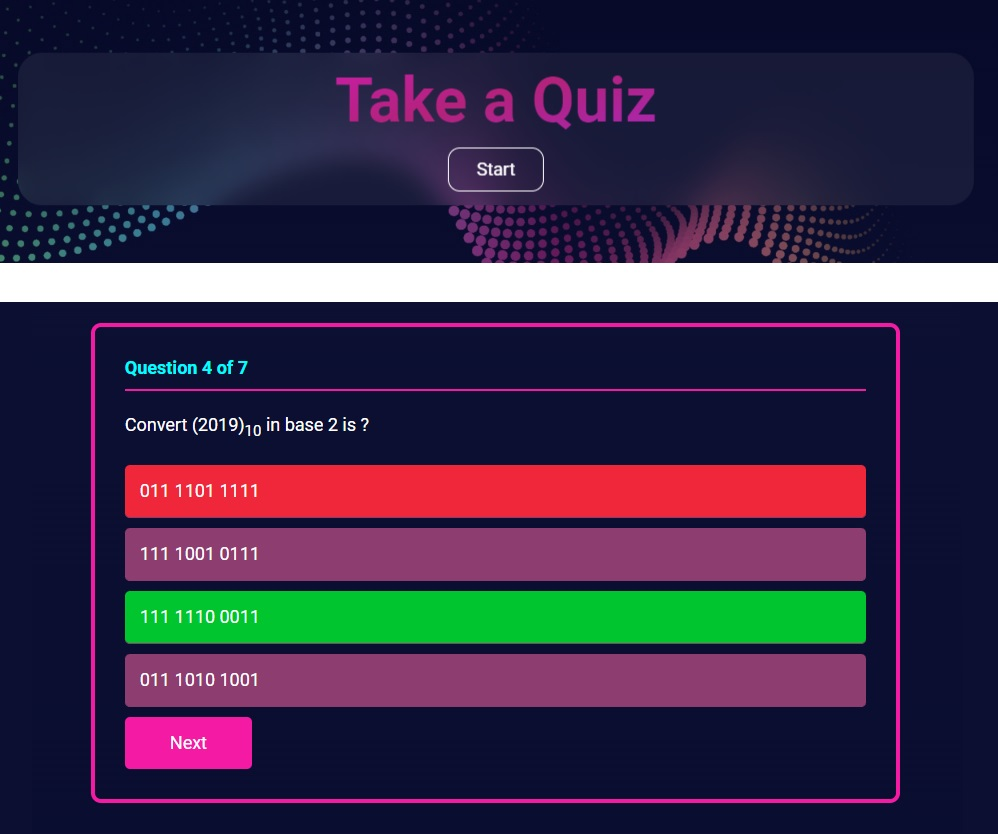
\includegraphics[scale=0.6]{img/29.jpg}                
	\caption{Quiz page} 
	\label{fig:quiz}
\end{figure*} 

\newpage
\subsection{Test interface}
The Test page is coming soon (see figure \ref{fig:test})

\begin{figure*}[ht]
	\centering
	\label{}
\includegraphics[scale=0.6]{img/30.jpg}                
	\caption{Test page coming soon} 
	\label{fig:test}
\end{figure*} 

\section{Hosting}
We are hosting the website at github pages at : https://lyes07.github.io/strm-website/index.html\\
and also at : http://coursstrm.epizy.com/
\\\\But hopefull in the future we will buy the domain name : coursstrm.com , so you can find the website at : http://coursstrm.com/
\section{Conclusion}
In this chapter, we have given a brief and clear clarification of the programming dialects utilized in creating of the website and the programs that were utilized without overlooking the devices utilized, and we too touched and showed the different interfaces,functions and given a clear clarification of the foremost imperative highlights of the website.\\